%%%%%%%%%%%%%%%%%%%%%%%%%%%%%%%%%%%%%%%%%%%%%%%%%%%%%%%%%%%%%%%%%
\phantomsection
\chapter{FLOW PREDICTION}\label{ch:fp}
%%%%%%%%%%%%%%%%%%%%%%%%%%%%%%%%%%%%%%%%%%%%%%%%%%%%%%%%%%%%%%%%%

\vspace{-12pt} %iki başlık alt alta. iki katı boşluk olmasın

\section{Purpose}

Lorem ipsum dolor sit amet, consectetur adipiscing elit. Sed ac augue vel dui 
adipiscing placerat et nec metus. Donec bibendum sodales mollis. Cras in lacus 
justo, at vestibulum quam. Sed semper, est sit amet consectetur ornare, leo est 
lacinia velit, adipiscing elementum lectus felis at sem. Aenean hendrerit erat eu 
lacus malesuada at sodales arcu egestas. Maecenas euismod urna ut sem luctus et 
congue metus vulputate. Ut pellentesque, neque eget fringilla elementum, ligula 
massa aliquet lorem, et varius nisi lacus vel diam. Etiam vitae metus sed orci 
rutrum fringilla. Phasellus sed velit quam. Mauris vestibulum, mauris a cursus 
adipiscing, nulla est hendrerit justo, ut fringilla eros velit ut mauris.

Sed et est vestibulum felis sagittis congue. Phasellus fringilla sem eu purus 
posuere ut viverra massa dignissim. Maecenas ornare neque velit. Vivamus interdum 
euismod elementum. Ut sit amet luctus ligula. Vivamus porttitor venenatis sem nec 
congue. Quisque sed lectus et nibh imperdiet vestibulum. Vivamus vel turpis leo. 
Proin suscipit iaculis nibh, nec dictum augue aliquet in. Praesent fermentum sem 
tempus orci molestie at facilisis dui sagittis. Etiam sit amet imperdiet sapien. 

\subsection{Artificial neural networks}

Lorem ipsum dolor sit amet, consectetur adipiscing elit. Sed ac augue vel dui 
adipiscing placerat et nec metus. Donec bibendum sodales mollis. Cras in lacus 
justo, at vestibulum quam. Sed semper, est sit amet consectetur ornare, leo est 
lacinia velit, adipiscing elementum lectus felis at sem. Aenean hendrerit erat eu 
lacus malesuada at sodales arcu egestas. Maecenas euismod urna ut sem luctus et 
congue metus vulputate.

\begin{figure}[!ht]
 \centering
 
\includegraphics[width=230pt,keepaspectratio=true]{./fig/sekil3}
 % sekil3.eps: 0x0 pixel, 300dpi, 0.00x0.00 cm, bb=14 14 1155 740
 \vspace*{4mm}
 \caption[Short version for LoF]{Long version to appear next to the figure.}
 \label{fig:3-1-1}
\end{figure}

Lorem ipsum dolor sit amet, consectetur adipiscing elit. Sed ac augue vel dui 
adipiscing placerat et nec metus. Donec bibendum sodales mollis. Cras in lacus 
justo, at vestibulum quam. Sed semper, est sit amet consectetur ornare, leo est 
lacinia velit, adipiscing elementum lectus felis at sem. Aenean hendrerit erat eu 
lacus malesuada at sodales arcu egestas. Maecenas euismod urna ut sem luctus et 
congue metus vulputate. Ut pellentesque, neque eget fringilla elementum, ligula 
massa aliquet lorem, et varius nisi lacus vel diam. Etiam vitae metus sed orci 
rutrum fringilla. Phasellus sed velit quam. Mauris vestibulum, mauris a cursus 
adipiscing, nulla est hendrerit justo, ut fringilla eros velit ut mauris.

Sed et est vestibulum felis sagittis congue. Phasellus fringilla sem eu purus 
posuere ut viverra massa dignissim. Maecenas ornare neque velit. Vivamus interdum 
euismod elementum. Ut sit amet luctus ligula. Vivamus porttitor venenatis sem nec 
congue. Quisque sed lectus et nibh imperdiet vestibulum. Vivamus vel turpis leo. 
Proin suscipit iaculis nibh, nec dictum augue aliquet in. Praesent fermentum sem 
tempus orci molestie at facilisis dui sagittis. Etiam sit amet imperdiet sapien.

\subsection{Autoregressive models}

Lorem ipsum dolor sit amet, consectetur adipiscing elit. Sed ac augue vel dui 
adipiscing placerat et nec metus. Donec bibendum sodales mollis. Cras in lacus 
justo, at vestibulum quam. Sed semper, est sit amet consectetur ornare, leo est 
lacinia velit, adipiscing elementum lectus felis at sem. Aenean hendrerit erat eu 
lacus malesuada at sodales arcu egestas defined in (\ref{eq:3-1}) 

\begin{equation}
\label{eq:3-1}
   y_{t}  \equiv \phi_{1} y_{t-1} + \epsilon_{t}
\end{equation}

Long and complex equation example in (\ref{eq:appendix}). Maecenas euismod urna ut sem luctus et congue metus vulputate. Ut pellentesque, neque eget fringilla elementum, ligula 
massa aliquet lorem, et varius nisi lacus vel diam. Etiam vitae metus sed orci 
rutrum fringilla. Phasellus sed velit quam. Mauris vestibulum, mauris a cursus 
adipiscing, nulla est hendrerit justo, ut fringilla eros velit ut mauris.

\subsection{Process based model: SWAT}

Lorem ipsum dolor sit amet, consectetur adipiscing elit. Sed ac augue vel dui 
adipiscing placerat et nec metus. Donec bibendum sodales mollis. Cras in lacus 
justo, at vestibulum quam. Sed semper, est sit amet consectetur ornare, leo est 
lacinia velit, adipiscing elementum lectus felis at sem. Aenean hendrerit erat eu 
lacus malesuada at sodales arcu egestas. Maecenas euismod urna ut sem luctus et 
congue metus vulputate. Ut pellentesque, neque eget fringilla elementum, ligula 
massa aliquet lorem, et varius nisi lacus vel diam. Etiam vitae metus sed orci 
rutrum fringilla. Phasellus sed velit quam. Mauris vestibulum, mauris a cursus 
adipiscing, nulla est hendrerit justo, ut fringilla eros velit ut mauris.

Sed et est vestibulum felis sagittis congue. Phasellus fringilla sem eu purus 
posuere ut viverra massa dignissim. Maecenas ornare neque velit. Vivamus interdum 
euismod elementum. Ut sit amet luctus ligula. Vivamus porttitor venenatis sem nec 
congue. Quisque sed lectus et nibh imperdiet vestibulum. Vivamus vel turpis leo. 
Proin suscipit iaculis nibh, nec dictum augue aliquet in. Praesent fermentum sem 
tempus orci molestie at facilisis dui sagittis. Etiam sit amet imperdiet sapien.

\begin{figure}[!ht]
 \centering
 
\includegraphics[width=230pt,keepaspectratio=true]{./fig/sekil3}
 % sekil3.eps: 0x0 pixel, 300dpi, 0.00x0.00 cm, bb=14 14 1155 740
 \vspace{4mm}
 \caption{For a multi-line figure captions, it is important that all the lines of the caption are aligned.}
 \label{fig:3-1-3}
\end{figure}

Figure~\ref{fig:3-1-3} shows that lorem ipsum dolor sit amet, consectetur adipiscing elit. Sed ac augue vel dui 
adipiscing placerat et nec metus. Donec bibendum sodales mollis. Cras in lacus 
justo, at vestibulum quam. Sed semper, est sit amet consectetur ornare, leo est 
lacinia velit, adipiscing elementum lectus felis at sem. Aenean hendrerit erat eu 
lacus malesuada at sodales arcu egestas. Maecenas euismod urna ut sem luctus et 
congue metus vulputate. Ut pellentesque, neque eget fringilla elementum, ligula 
massa aliquet lorem, et varius nisi lacus vel diam. Etiam vitae metus sed orci 
rutrum fringilla. Phasellus sed velit quam. Mauris vestibulum, mauris a cursus 
adipiscing, nulla est hendrerit justo, ut fringilla eros velit ut mauris.

Sed et est vestibulum felis sagittis congue. Phasellus fringilla sem eu purus 
posuere ut viverra massa dignissim. Maecenas ornare neque velit. Vivamus interdum 
euismod elementum. Ut sit amet luctus ligula. Vivamus porttitor venenatis sem nec 
congue. Quisque sed lectus et nibh imperdiet vestibulum. Vivamus vel turpis leo. 
Proin suscipit iaculis nibh, nec dictum augue aliquet in. Praesent fermentum sem 
tempus orci molestie at facilisis dui sagittis. Etiam sit amet imperdiet sapien.

\subsection{Multi variable analysis}

Lorem ipsum dolor sit amet, consectetur adipiscing elit. Sed ac augue vel dui 
adipiscing placerat et nec metus. Donec bibendum sodales mollis. Cras in lacus 
justo, at vestibulum quam. Sed semper, est sit amet consectetur ornare, leo est 
lacinia velit, adipiscing elementum lectus felis at sem. Aenean hendrerit erat eu 
lacus malesuada at sodales arcu egestas. Maecenas euismod urna ut sem luctus et 
congue metus vulputate. Ut pellentesque, neque eget fringilla elementum, ligula 
massa aliquet lorem, et varius nisi lacus vel diam. Etiam vitae metus sed orci 
rutrum fringilla. Phasellus sed velit quam. Mauris vestibulum, mauris a cursus 
adipiscing, nulla est hendrerit justo, ut fringilla eros velit ut mauris.

Sed et est vestibulum felis sagittis congue. Phasellus fringilla sem eu purus 
posuere ut viverra massa dignissim. Maecenas ornare neque velit. Vivamus interdum 
euismod elementum. Ut sit amet luctus ligula. Vivamus porttitor venenatis sem nec 
congue. Quisque sed lectus et nibh imperdiet vestibulum. Vivamus vel turpis leo. 
Proin suscipit iaculis nibh, nec dictum augue aliquet in. Praesent fermentum sem 
tempus orci molestie at facilisis dui sagittis. Etiam sit amet imperdiet sapien illustrated in Figure~\ref{fig:3-1-4}.

\begin{figure}[!ht]
 \centering
 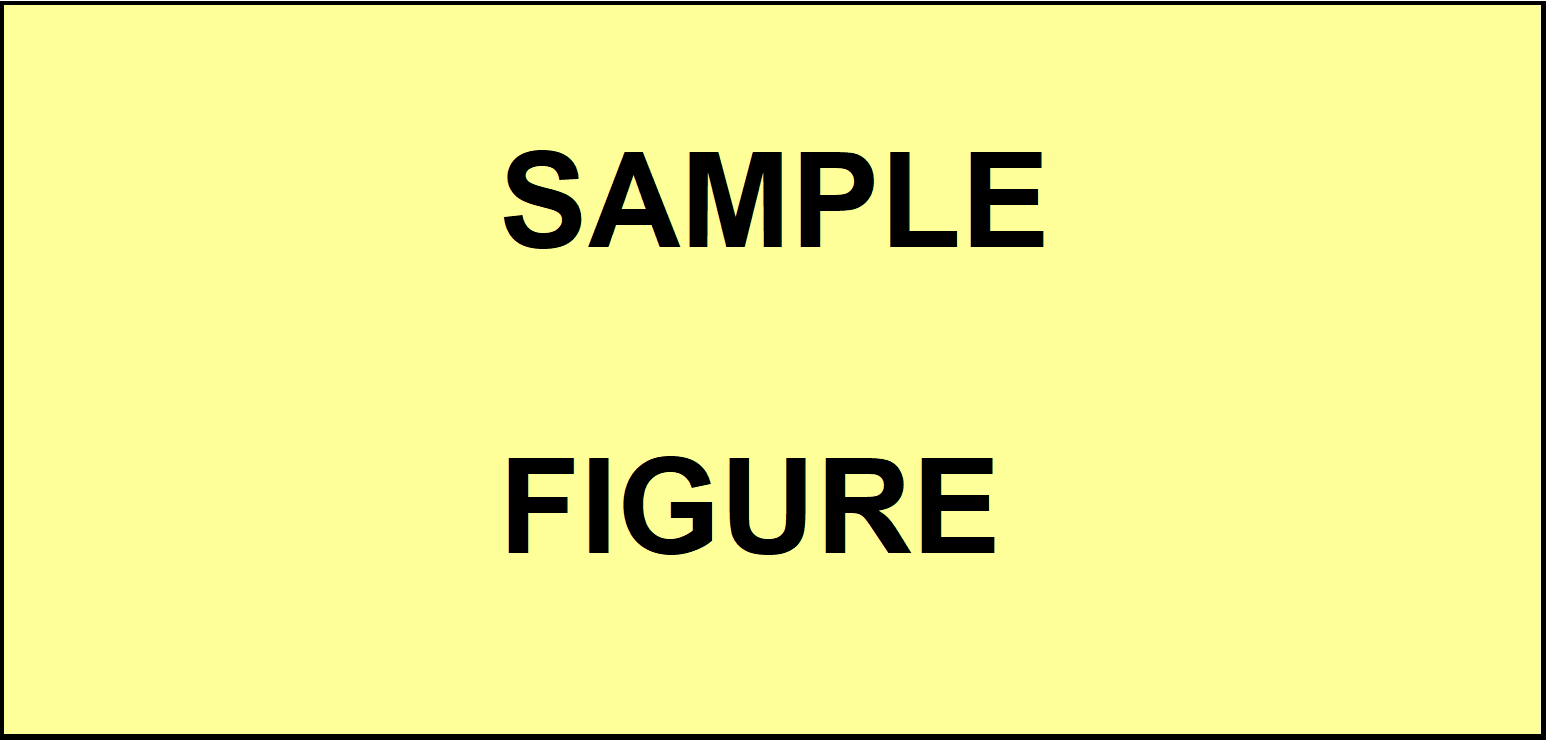
\includegraphics[width=290pt,keepaspectratio=true]{./fig/sekil4}
 % sekil4.eps: 0x0 pixel, 300dpi, 0.00x0.00 cm, bb=14 14 1148 603
 \vspace{4mm}
 \caption{Figure captions must be ended with a full stop.}
 \label{fig:3-1-4}
\end{figure}

Lorem ipsum dolor sit amet, consectetur adipiscing elit. Sed ac augue vel dui 
adipiscing placerat et nec metus. Donec bibendum sodales mollis. Cras in lacus 
justo, at vestibulum quam. Sed semper, est sit amet consectetur ornare, leo est 
lacinia velit, adipiscing elementum lectus felis at sem. Aenean hendrerit erat eu 
lacus malesuada at sodales arcu egestas. Maecenas euismod urna ut sem luctus et 
congue metus vulputate. Ut pellentesque, neque eget fringilla elementum, ligula 
massa aliquet lorem, et varius nisi lacus vel diam. Etiam vitae metus sed orci 
rutrum fringilla. Phasellus sed velit quam. Mauris vestibulum, mauris a cursus 
adipiscing, nulla est hendrerit justo, ut fringilla eros velit ut mauris in (\ref{equation_3_2}).
\begin{equation}
    D\left(C_{A},C_{B}\right) = \min X_{A}\in C_{A},X_{B}\in C_{B} 
     d\left(X_{A},X_{B}\right)  
     \label{equation_3_2}
\end{equation}
Sed et est vestibulum felis sagittis congue. Phasellus fringilla sem eu purus 
posuere ut viverra massa dignissim. Maecenas ornare neque velit. Vivamus interdum 
euismod elementum. Ut sit amet luctus ligula. Vivamus porttitor venenatis sem nec 
congue. Quisque sed lectus et nibh imperdiet vestibulum. Vivamus vel turpis leo. 
Proin suscipit iaculis nibh, nec dictum augue aliquet in. Praesent fermentum sem 
tempus orci molestie at facilisis dui sagittis. Etiam sit amet imperdiet sapien. Figure~\ref{fig:landscape_figure} is a landscape image example.

\begin{landscape}
\thispagestyle{empty}
 \begin{figure}[!ht]
 \vspace{-2mm}
 \centering
 
\includegraphics[width=450pt,keepaspectratio=true]{./fig/sekil3}
 % sekil3.eps: 0x0 pixel, 300dpi, 0.00x0.00 cm, bb=14 14 1155 740
 \vspace{4mm}
 \caption{Landscape-oriented, full-page figure.}    
      \vspace{40mm} % You can adjust the position of the page number. (Change 45mm to the value you want.)
      \hspace{0cm}\pageref{fig:landscape_figure}   %ATTENTION!! The figure label name and the label name used in \pageref must be identical for the page number to display correctly!
      \label{fig:landscape_figure}
\end{figure}
\end{landscape}

\section{Practical Applications}

Lorem ipsum dolor sit amet, consectetur adipiscing elit. Sed ac augue vel dui 
adipiscing placerat et nec metus. Donec bibendum sodales mollis. Cras in lacus 
justo, at vestibulum quam. Sed semper, est sit amet consectetur ornare, leo est 
lacinia velit, adipiscing elementum lectus felis at sem. Aenean hendrerit erat eu 
lacus malesuada at sodales arcu egestas. Maecenas euismod urna ut sem luctus et 
congue metus vulputate. Ut pellentesque, neque eget fringilla elementum, ligula 
massa aliquet lorem, et varius nisi lacus vel diam. Etiam vitae metus sed orci 
rutrum fringilla. Phasellus sed velit quam. Mauris vestibulum, mauris a cursus 
adipiscing, nulla est hendrerit justo, ut fringilla eros velit ut mauris.

Lorem ipsum dolor sit amet, consectetur adipiscing elit. Sed ac augue vel dui 
adipiscing placerat et nec metus. Donec bibendum sodales mollis. Cras in lacus 
justo, at vestibulum quam. Sed semper, est sit amet consectetur ornare, leo est 
lacinia velit, adipiscing elementum lectus felis at sem. Aenean hendrerit erat eu 
lacus malesuada at sodales arcu egestas. Maecenas euismod urna ut sem luctus et 
congue metus vulputate. Ut pellentesque, neque eget fringilla elementum, ligula 
massa aliquet lorem, et varius nisi lacus vel diam.

\section{Application Data}

Lorem ipsum dolor sit amet, consectetur adipiscing elit. Sed ac augue vel dui 
adipiscing placerat et nec metus. Donec bibendum sodales mollis. Cras in lacus 
justo, at vestibulum quam. Sed semper, est sit amet consectetur ornare, leo est 
lacinia velit, adipiscing elementum lectus felis at sem. Aenean hendrerit erat eu 
lacus malesuada at sodales arcu egestas. Maecenas euismod urna ut sem luctus et 
congue metus vulputate. Ut pellentesque, neque eget fringilla elementum, ligula 
massa aliquet lorem, et varius nisi lacus vel diam. Etiam vitae metus sed orci 
rutrum fringilla. Phasellus sed velit quam. Mauris vestibulum, mauris a cursus 
adipiscing, nulla est hendrerit justo, ut fringilla eros velit ut mauris.

Lorem ipsum dolor sit amet, consectetur adipiscing elit. Sed ac augue vel dui 
adipiscing placerat et nec metus. Donec bibendum sodales mollis. Cras in lacus 
justo, at vestibulum quam. Sed semper, est sit amet consectetur ornare, leo est 
lacinia velit, adipiscing elementum lectus felis at sem. Aenean hendrerit erat eu 
lacus malesuada at sodales arcu egestas. Maecenas euismod urna ut sem luctus et 
congue metus vulputate. Ut pellentesque, neque eget fringilla elementum, ligula 
massa aliquet lorem, et varius nisi lacus vel diam. Etiam vitae metus sed orci 
rutrum fringilla. Phasellus sed velit quam. Mauris vestibulum, mauris a cursus 
adipiscing, nulla est hendrerit justo, ut fringilla eros velit ut mauris
\cite{Wegener2000629}.

% ---------------------------------------------------------------- %
% Numbered citation.						   %
% ---------------------------------------------------------------- %

Lorem ipsum dolor sit amet, consectetur adipiscing elit. Sed ac augue vel dui 
adipiscing placerat et nec metus \cite{Wolchik2000843}. 
Donec bibendum sodales mollis. Cras in lacus 
justo, at vestibulum quam. Sed semper, est sit amet consectetur ornare, leo est 
lacinia velit, adipiscing elementum lectus felis at sem. Aenean hendrerit erat eu 
lacus malesuada at sodales arcu egestas. Maecenas euismod urna ut sem luctus et 
congue metus vulputate. Ut pellentesque, neque eget fringilla elementum, ligula 
massa aliquet lorem, et varius nisi lacus vel diam. Etiam vitae metus sed orci 
rutrum fringilla. Phasellus sed velit quam \cite{Zuckerman199486}. 
Mauris vestibulum, mauris a cursus 
adipiscing, nulla est hendrerit justo, ut fringilla eros velit ut mauris. Table~\ref{table:landscape_table1} is an example of landscape table. Table~\ref{table:landscape_table1} (continued) is an example of continued landscape table. If this does not exist in your case, remove it.

% ---------------------------------------------------------------- %
% Page numbers must be on the bottom-middle of short side (when    %
% portrait-oriented), or bottom-middle of long side (when	   %
% landscape-oriented)						   %
% -----------------------------------------
\begin{landscape}
\thispagestyle{empty}

\begin{table*}[!ht]
\vspace{-6mm}
{\setlength{\tabcolsep}{14pt}
\renewcommand{\arraystretch}{1.1} % Row spacing increased
\caption{Table writing in landscape-oriented pages:
The most important point is to align the rows horizontally.}
\begin{center}
\vspace{-6mm}
\begin{tabular}{|l|c|c|r|r|r|r|r|}
\hline
\multirow{2}{*}{Parameter} & \multirow{2}{*}{Column 2} & \multirow{2}{*}{Column 3} & \multicolumn{3}{|c|}{Column 4} & \multicolumn{2}{|c|}{Column 5}\\ \cline{4-8}
  & & & Subcolumn 1 & Subcolumn 2 & Subcolumn 3 & Subcolumn 4 & Subcolumn 5 \\
\hline
Row 1 & -7.680442 & 7.6986348 & 0.00 & 0.00 & 0.00 & 12 & 12 \\
Row 2 & 140 & - & 0.50 & 0.00 & 0.00 & 0 & 0 \\
Row 3 & 37.174357 & 37.16192697 & 0.00 & 0.00 & 0.00 & 0 & 24 \\
Row 4 & 140 & - & 0.50 & 0.00 & 0.00 & 0 & 0 \\
Row 5 & 37.174357 & 37.16192697 & 0.00 & 0.00 & 0.00 & 0 & 24 \\
Row 6 & 140 & - & 0.50 & 0.00 & 0.00 & 0 & 0 \\
Row 7 & 37.174357 & 37.16192697 & 0.00 & 0.00 & 0.00 & 0 & 24 \\
Row 8 & 140 & - & 0.50 & 0.00 & 0.00 & 0 & 0 \\
Row 9 & 37.174357 & 37.16192697 & 0.00 & 0.00 & 0.00 & 0 & 24 \\
Row 10 & 140 & - & 0.50 & 0.00 & 0.00 & 0 & 0 \\
Row 11 & 37.174357 & 37.16192697 & 0.00 & 0.00 & 0.00 & 0 & 24 \\
Row 12 & 140 & - & 0.50 & 0.00 & 0.00 & 0 & 0 \\
Row 13 & 37.174357 & 37.16192697 & 0.00 & 0.00 & 0.00 & 0 & 24 \\
Row 14 & 140 & - & 0.50 & 0.00 & 0.00 & 0 & 0 \\
Row 15 & 37.174357 & 37.16192697 & 0.00 & 0.00 & 0.00 & 0 & 24 \\
\hline
\end{tabular}
\end{center}
\begin{center}
      \vspace{40mm}     % You can adjust the position of the page number. (Change 15mm to the value you want.)
      \hspace{0cm}\pageref{table:landscape_table1}
      \label{table:landscape_table1}
\end{center}
}
\end{table*}
\end{landscape}

% If the table continues, it is continued from the new page as below.


\begin{landscape}
\thispagestyle{empty}
\begin{table*}[!htb]
\vspace{6mm}
{\setlength{\tabcolsep}{14pt}
\renewcommand{\arraystretch}{1.1} % Increased row spacing
\caption*{{\bf Table~\ref{table:landscape_table1} (continued) :} An example table name that continues to the second row, an example table name that continues to the second row, an example table name that continues to the second row, an example table name that continues to the second row.}
\begin{center}
\vspace{-6mm}
\begin{tabular}{|l|c|c|r|r|r|r|r|}
\hline
\multirow{2}{*}{Parameter} & \multirow{2}{*}{Column 2} & \multirow{2}{*}{Column 3} & \multicolumn{3}{|c|}{Column 4} & \multicolumn{2}{|c|}{Column 5}\\ \cline{4-8}
  & & & Subcolumn 1 & Subcolumn 2 & Subcolumn 3 & Subcolumn 4 & Subcolumn 5 \\
\hline
Row 16 & -7.680442 & 7.6986348 & 0.00 & 0.00 & 0.00 & 12 & 12 \\
Row 17 & 140 & - & 0.50 & 0.00 & 0.00 & 0 & 0 \\
Row 18 & 37.174357 & 37.16192697 & 0.00 & 0.00 & 0.00 & 0 & 24 \\
Row 19 & 140 & - & 0.50 & 0.00 & 0.00 & 0 & 0 \\
Row 20 & 37.174357 & 37.16192697 & 0.00 & 0.00 & 0.00 & 0 & 24 \\
Row 21 & 140 & - & 0.50 & 0.00 & 0.00 & 0 & 0 \\
Row 22 & 37.174357 & 37.16192697 & 0.00 & 0.00 & 0.00 & 0 & 24 \\
Row 23 & 140 & - & 0.50 & 0.00 & 0.00 & 0 & 0 \\
\hline
\end{tabular}
\end{center}
\begin{center}
      \vspace{70mm}    % You can adjust the position of the page number. (Change 15mm to the value you want.)
      \hspace{0cm}\pageref{table:landscape_table1_cont}
      \label{table:landscape_table1_cont}
\end{center}
}
\end{table*}
\end{landscape}
